% This is LLNCS.DEM the demonstration file of
% the LaTeX macro package from Springer-Verlag
% for Lecture Notes in Computer Science,
% version 2.4 for LaTeX2e as of 16. April 2010
%
\documentclass{llncs}
%
\usepackage{makeidx}  % allows for indexgeneration
\usepackage{graphicx} % for importing images
\usepackage{url} % for URL references
\usepackage{float}
% used for drawing the diagrams
\usepackage{tikz}
\usetikzlibrary{calc,trees,positioning,arrows,chains,shapes.geometric,%
    decorations.pathreplacing,decorations.pathmorphing,shapes,%
    matrix,shapes.symbols}

% defining diagram's style, just in case
\tikzset{
>=stealth',
  arrow/.style={
    rectangle, 
    rounded corners, 
    % fill=black!10,
    draw=black, very thick,
    text width=10em, 
    minimum height=3em, 
    text centered, 
    on chain},
  line/.style={draw, thick, <-},
  element/.style={
    tape,
    top color=white,
    bottom color=blue!50!black!60!,
    minimum width=8em,
    draw=blue!40!black!90, very thick,
    text width=10em, 
    minimum height=3.5em, 
    text centered, 
    on chain},
  every join/.style={->, thick,shorten >=1pt},
  decoration={brace},
  tuborg/.style={decorate},
  tubnode/.style={midway, right=2pt},
}
%
\begin{document}
%
%

%


%
\mainmatter              % start of the contributions
\pagestyle{headings}

%
\title{Automatic News Generation Based on Twitter}
%
\titlerunning{Automatic News Generation Based on Twitter}  % abbreviated title (for running head)
%                                     also used for the TOC unless
%                                     \toctitle is used
%
\author{Ali Alavi\inst{1} \and Rolf Jagerman\inst{1} \and
Tsay Kai-En\inst{1}}
%
\authorrunning{Ali Alavi, Rolf Jagerman and Tsay Kai-En} % abbreviated author list (for running head)
%
%
\institute{ETH Z\"urich, Z\"urich, Switzerland\\
\email{alavis@ethz.ch, \{rolfj, tsayk\}@student.ethz.ch}
}

\maketitle              % typeset the title of the contribution
%
\section{Introduction}
%
This report presents the current status of the project \textbf{Automatic News Generation Based on Twitter}, 
for \textbf{Big Data} course (code \textit{263-3010-00L}). This project tries to answer the following questions: 
\textit{Can we automatically generate news headlines based on public twitter posts? Can this method of news generation 
perform better than the available news agencies, in terms of speed, reliability and so on?}

We tackle this problem by taking the following steps:

\begin{enumerate}
  \item \textit{Data collection: }Gathering a large set of twitter posts and news headlines 
  \item \textit{Building a classifier: }Use the news headlines to train a classifier
  \item \textit{Labeling the tweets: }Label each tweet using the classifier we previously trained
\end{enumerate}


In the rest of this report we elaborate these steps in more details.

\section{Data collection}
\subsection{Data sources}
\subsubsection{Twitter data}
Twitter offer different ways of gathering data for different applications ~\cite{twitterdocumentation}. Unfortunately, giving access to the historic data is not one of them. In other words, our access to public data is limited to the most recent tweets. Hence, we decided to collect a large number of the most recent public tweets. 
Although Twitter Firehose ~\cite{twitterrestapi} offers access to all public tweets, it requires special permission to access, which we could not aquire. Luckily, Twitter's \textit{Streaming API} ~\cite{twitterstreaming} can offer a large number of tweets: it streams a random subset (around one percent) of all the public tweets. this subset is large enough for our purpose. Moreover, the streaming API allows for a much faster collection of tweets in comparison to other APIs such as \textit{REST API}, and also does not have the rate limitations imposed by Twitter on its \textit{REST} APIs ~\cite{twitterdocumentation}. 


\subsubsection{News data}
We looked into different news agencies (CNN, BBC, USA Today, The New York Times,...) and news aggregators (Feedzilla, Google News, Bing Search, ...) in order to collect the required data for training the classifier. Unfortunately, all such sources impose some rather strict limitations on the number of requests and results an agent can send and recieve. As an example, Feedzilla has a limitation of 100 results per request. Bing news is also a commercial product costs of which we cannot afford! ~\cite{bingsearchapi}. Although we managed to collect a good amount of news using The New Your Times ~\cite{thenytimes} and USA Today ~\cite{thenytimes} APIs, we gave them up for a better news source: Twitter accounts of the news agencies. 

All news agencies that we looked for have different twitter accounts for different news categories. For the first phase of the project, we chose to use the following news categories:

\begin{enumerate}
  \item Politics
  \item Sports
  \item Technology
\end{enumerate}

These categories are chosen due to the following facts:
\begin{itemize}
  \item There is not much overlap between these news categories (cf. business, technology, finance)
  \item The frequency of the news generated in these categories are significantly higher that other categories (couple of news every hour)
\end{itemize}


\subsection{Data storage}
To use the streaming API, the data collecting script needs to send an initial request and then keep listening for the stream of responses. Thus, we need to keep the script running on a server, for a long period of time. Moreover, the API publishes more than 2000 tweets per second. This translates to around 20 gigabytes of tweets per day. This imposes a data storage problem, as our resources were rather limited at the first phase of the project. In order to address these issues, we managed to use one of the school's servers to run our script on. This server had around 200 GB of free space, which allows for almost 10 days of continous data collection. Moreover, we managed to use RAR compression to reduce the data size by a factor of 7. Moreover, since school servers are not the most reliable type of servers, we decided to take precautions by setting up a home-based Raspberry Pi ~\cite{wiki:raspberrypi} server and connecting it to a 1-terabyte external hard disk drive (See Figure ~\ref{fig:Raspberry Pi}). Using this setup, we are capable of collecting and storing around 350 days of twitter data using the \textit{Streaming API}:
\[\textit{Days of tweet collection}=\frac{\textit{Storage size}\times \textit{Compression ratio}} {\textit{Size of tweets per day}}\]
\[\frac{\textit{1000 GB} \times 7}{\textit{20 GB per day}}=\textit{350 days} \]

\begin{figure}[H]
  \centering
  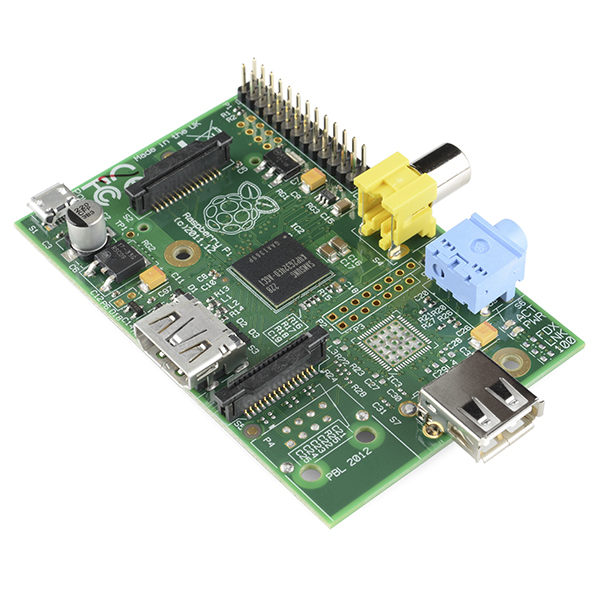
\includegraphics[width=0.5\textwidth]{images/rpi.jpg}
  \caption{Raspberry Pi Setup / Image to be updated by Ali}
  \label{fig:Raspberry Pi}
\end{figure}

\section{How to train your classifier}

[CONTENT BY ROLF \& ALI]

A detailed diagram of the system is seen in Figure \ref{fig:System diagram}.

\begin{figure}[H]
  \centering
  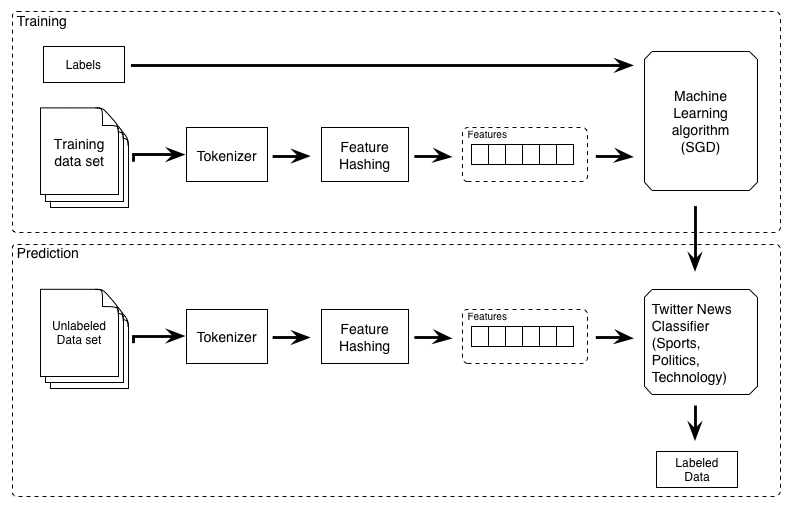
\includegraphics[width=\textwidth]{images/system.png}
  \caption{System diagram}
  \label{fig:System diagram}
\end{figure}

\section{Tools, Languages and Libraries}
Python was used as the sole programming language of the project.
In later steps we might use Java or Scala to scale the project.
We used the Python machine learning package Scikit ~\cite{scikit-learn}, which significantly simplified development of the trainer. 


\bibliographystyle{plain}
\bibliography{report.bib}

\end{document}